%%%%%%%%%%%%%%%%%%%%%%
%\appendix[Appendix A: Example I]{Appendix A: Example I} 
\appendix[Waveform, spectrogram and SNR of frog species from trophy recordings]{Waveform, spectrogram and SNR of frog species from trophy recordings} 



\begin{table}[htb!]
\centering
\caption[Waveform, spectrogram, and SNR of trophy recordings]{Waveform, spectrogram, and SNR of selected six frog species from trophy recordings. The SNR is calculated as 
$SNR=10 \times log_{10}[(\sum_{i=m}^{m+L}S_{i}^2)/(\sum_{j=n}^{n+L}N_{j}^2)]$
, where $L$ is the length of the signal and noise used for calculating SNR, and set at 6000 samples, $n$ and $m$ are manually selected start location in the waveform for noise and signal, respectively}
\label{tab:wav_spec_cd}
\begin{tabular}{llll}
\hline\hline
       & Waveform & Spectrogram & SNR (dB)   \\ \hline
\textit{Bufo marinus}        &   
\begin{minipage}{.3\textwidth} 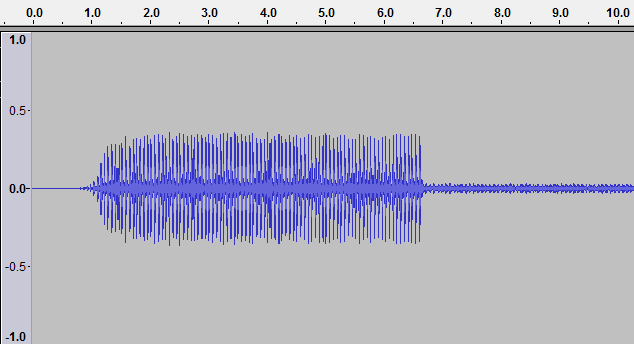
\includegraphics[width=45mm, height=30mm]{image/Ch1/toad_wave.png}  \end{minipage}    &   \begin{minipage}{.3\textwidth} 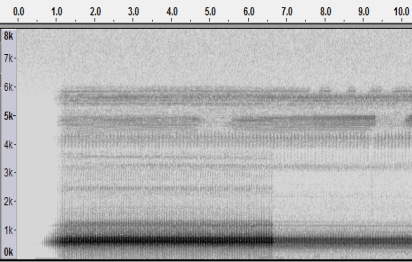
\includegraphics[width=45mm, height=30mm]{image/Ch1/toad_spec.png}  \end{minipage}          & 19.35 \\ \hline
\textit{Litoria caerulea}    &  \begin{minipage}{.3\textwidth} 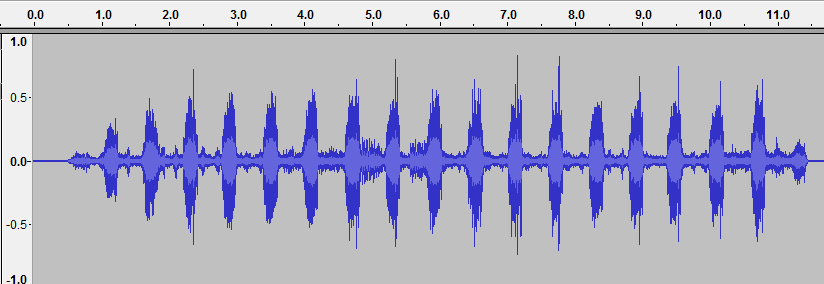
\includegraphics[width=45mm, height=30mm]{image/Ch1/caerulea_wav.png}  \end{minipage}      &     \begin{minipage}{.3\textwidth} 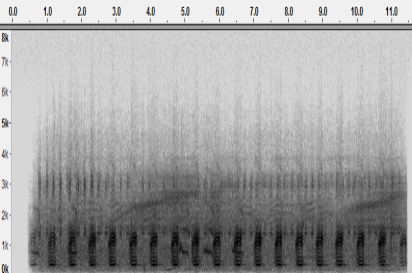
\includegraphics[width=45mm, height=30mm]{image/Ch1/caerulea_spec.png}   \end{minipage}     & 15.78 \\ \hline
\textit{Litoria fallax}      &      \begin{minipage}{.3\textwidth} 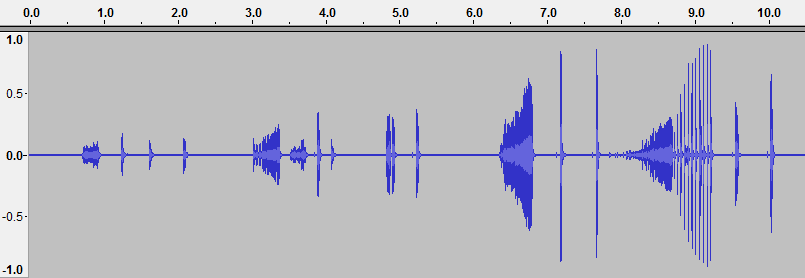
\includegraphics[width=45mm, height=30mm]{image/Ch1/fallax_wav.png} \end{minipage}   &   \begin{minipage}{.3\textwidth} 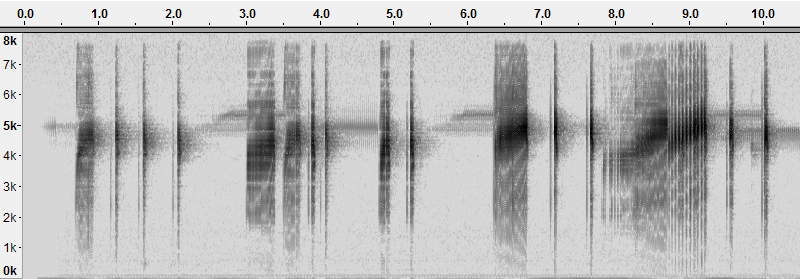
\includegraphics[width=45mm, height=30mm]{image/Ch1/fallax_spec.png}   \end{minipage}       & 43.7  \\ \hline
\end{tabular}
\end{table}





\begin{table}[ht!]
\centering
\begin{tabular}{llll}
\hline
\textit{Litoria gracillenta} &     \begin{minipage}{.3\textwidth} 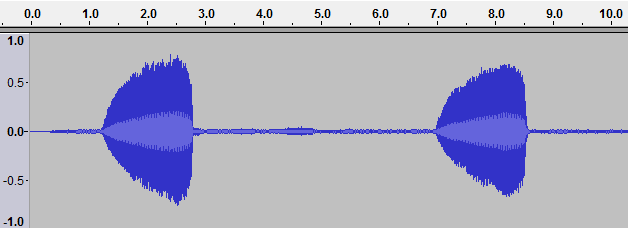
\includegraphics[width=45mm, height=30mm]{image/Ch1/graci_wav.png}  \end{minipage}   &    \begin{minipage}{.3\textwidth} 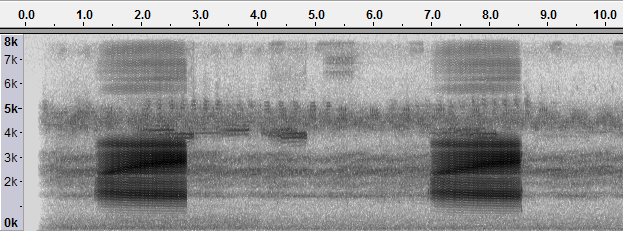
\includegraphics[width=45mm, height=30mm]{image/Ch1/graci_spec.png}     \end{minipage}    & 25.8  \\ \hline
\textit{Litoria latopalmata} &      \begin{minipage}{.3\textwidth} 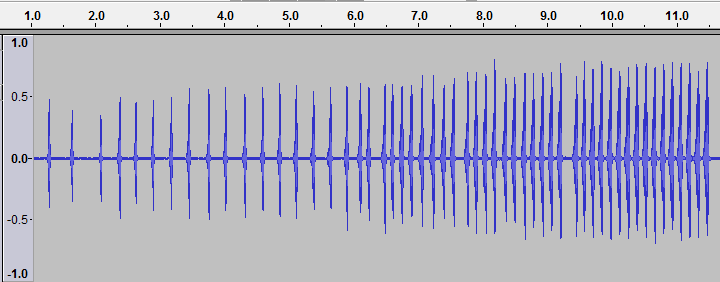
\includegraphics[width=45mm, height=30mm]{image/Ch1/latop_wav.png}  \end{minipage}  &    \begin{minipage}{.3\textwidth} 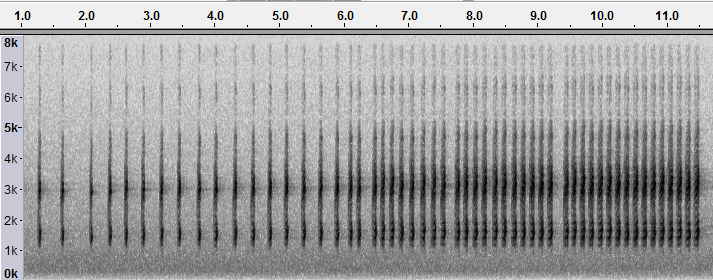
\includegraphics[width=45mm, height=30mm]{image/Ch1/latop_spec.png}    \end{minipage}     & 35.85 \\ \hline
\textit{Litoria rubella}     &   \begin{minipage}{.3\textwidth} 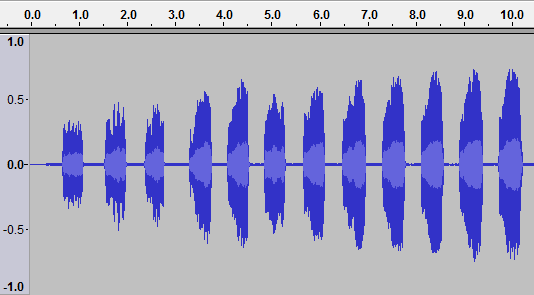
\includegraphics[width=45mm, height=30mm]{image/Ch1/rubella_wav.png}   \end{minipage}    &       \begin{minipage}{.3\textwidth} 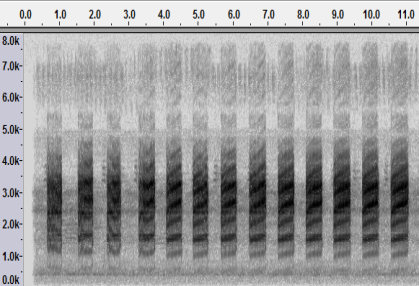
\includegraphics[width=45mm, height=30mm]{image/Ch1/rubella_spec.png}   \end{minipage}   & 36.2  \\ \hline\hline
\end{tabular}
\end{table}




\appendix[Waveform, spectrogram and SNR of eight frog species from field recordings]{Waveform, spectrogram and SNR of six frog species from field recordings} 

\begin{table}[htb!]
\centering
\caption[Waveform, spectrogram, and SNR of field recordings]{Waveform, spectrogram, and SNR of eight frog species (field recordings)}
\label{tab:JCU_para}
\resizebox{\textwidth}{!}{
\begin{tabular}{llll}
\hline\hline
                            & Waveform & Spectrogram & SNR (dB) \\ \hline
\textit{Bufo marinus}                &   \begin{minipage}{.3\textwidth} 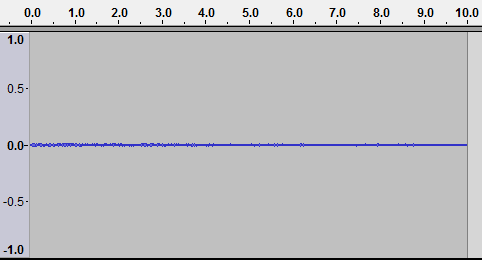
\includegraphics[width=45mm, height=30mm]{image/Ch1/toad_jcu_wav.png}  \end{minipage}       &      \begin{minipage}{.3\textwidth} 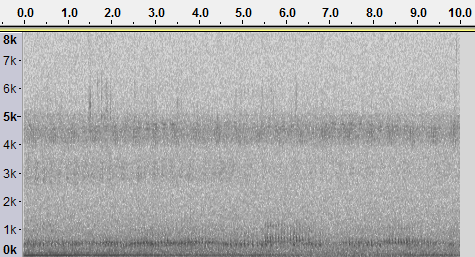
\includegraphics[width=45mm, height=30mm]{image/Ch1/toad_jcu_spec.png}  \end{minipage}       & 1.86     \\ \hline
\textit{Cyclorana novaehollandiae}   &  \begin{minipage}{.3\textwidth} 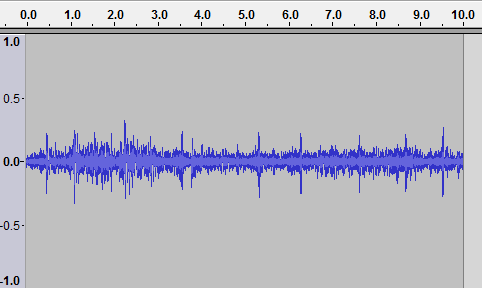
\includegraphics[width=45mm, height=30mm]{image/Ch1/cyc_jcu_wav.png}  \end{minipage}        & \begin{minipage}{.3\textwidth} 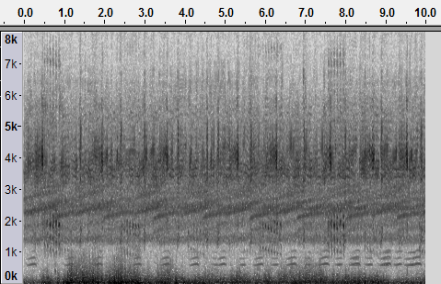
\includegraphics[width=45mm, height=30mm]{image/Ch1/cyc_jcu_spec.png}  \end{minipage}            & -0.13    \\ \hline
\textit{Limnodynastes terraereginae} &  \begin{minipage}{.3\textwidth} 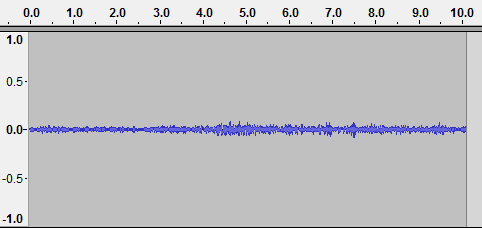
\includegraphics[width=45mm, height=30mm]{image/Ch1/ter_jcu_wav.png}  \end{minipage}        &   \begin{minipage}{.3\textwidth} 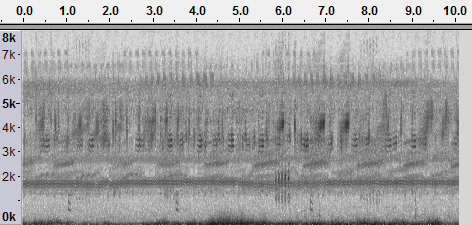
\includegraphics[width=45mm, height=30mm]{image/Ch1/ter_jcu_spec.png}  \end{minipage}          & -2.88    \\ \hline
\textit{Litoria fallax}              &   \begin{minipage}{.3\textwidth} 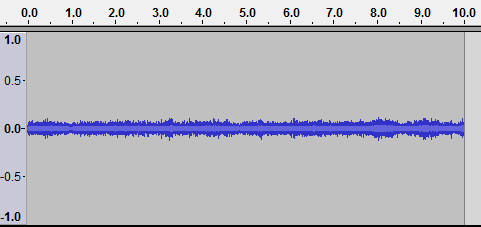
\includegraphics[width=45mm, height=30mm]{image/Ch1/fallax_jcu_wav.png}  \end{minipage}       &    \begin{minipage}{.3\textwidth} 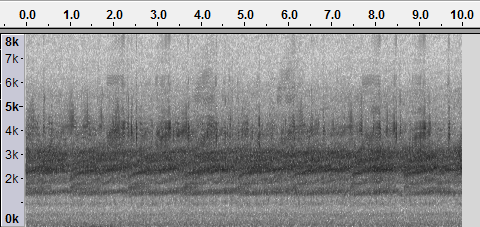
\includegraphics[width=45mm, height=30mm]{image/Ch1/fallax_jcu_spec.png}  \end{minipage}         & 1.52     \\ \hline
\end{tabular}
}
\end{table}


\begin{table}[htb!]
\centering
\resizebox{\textwidth}{!}{
\begin{tabular}{llll}
\hline
\textit{Litoria nasuta}              &   \begin{minipage}{.3\textwidth} 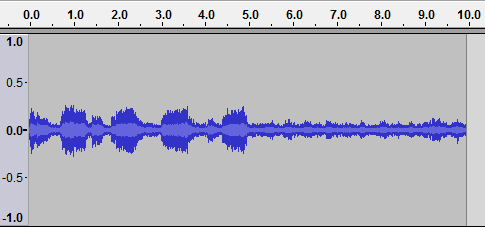
\includegraphics[width=45mm, height=30mm]{image/Ch1/nasuta_jcu_wav.png}  \end{minipage}       &  \begin{minipage}{.3\textwidth} 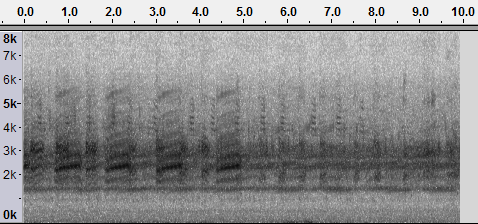
\includegraphics[width=45mm, height=30mm]{image/Ch1/nasuta_jcu_spec.png}  \end{minipage}           & 2.14     \\ \hline
\textit{Litoria rothii}              &   \begin{minipage}{.3\textwidth} 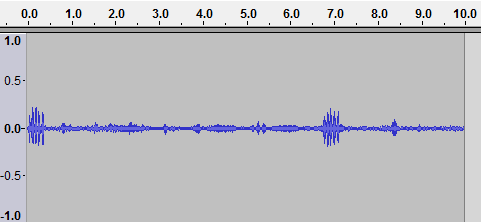
\includegraphics[width=45mm, height=30mm]{image/Ch1/rothii_jcu_wav.png}  \end{minipage}       &    \begin{minipage}{.3\textwidth} 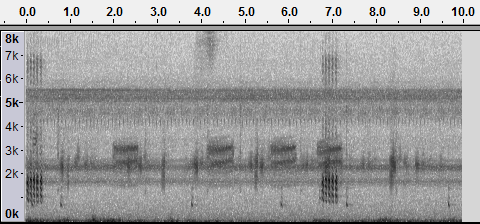
\includegraphics[width=45mm, height=30mm]{image/Ch1/rothii_jcu_spec.png}  \end{minipage}         & 10.24    \\ \hline
\textit{Litoria rubella}            &    \begin{minipage}{.3\textwidth} 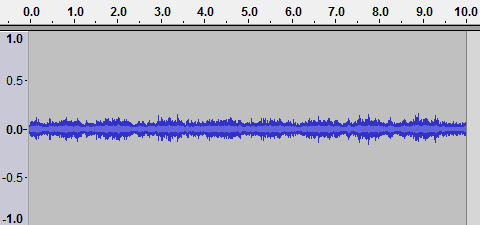
\includegraphics[width=45mm, height=30mm]{image/Ch1/rubella_jcu_wav.png}  \end{minipage}      &   \begin{minipage}{.3\textwidth} 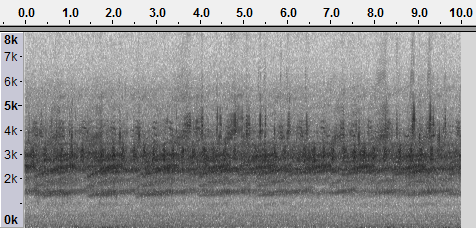
\includegraphics[width=45mm, height=30mm]{image/Ch1/rubella_jcu_spec.png}  \end{minipage}          & 1.08     \\ \hline
\textit{Uperolela mimula}            &   \begin{minipage}{.3\textwidth} 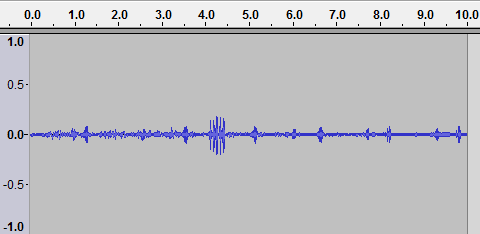
\includegraphics[width=45mm, height=30mm]{image/Ch1/mimula_jcu_wav.png}  \end{minipage}       &  \begin{minipage}{.3\textwidth} 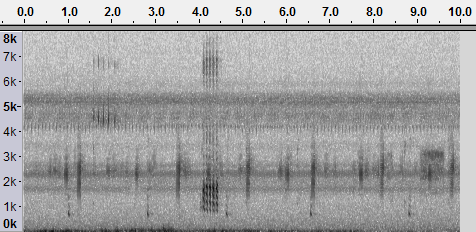
\includegraphics[width=45mm, height=30mm]{image/Ch1/mimula_jcu_spec.png}  \end{minipage}           & 10.28    \\ \hline\hline
\end{tabular}
}
\end{table}





\appendix[A overview of frog call classification performance]{An overview of frog call classification performance} 

\begin{table}[htb!]
\centering
\caption{A brief overview of frog call classification performance}
\label{tab:classificationPerformance}
\resizebox{\textwidth}{!}{
\Rotatebox{90}{%
\begin{tabular}{llll}
\hline\hline
\textbf{Database}                   & \textbf{Performance}                   & \textbf{Reference} & \textbf{Data source} \\ \hline

22 frog species &  NA  & \citet{grigg1996monitoring} & Collected from Queensland, Australia (unavailable) \\ 

4 frog species with 66 samples & \begin{tabular}[c]{@{}l@{}}  Best performance with averaged classification \\ Accuracy of 72.18\% and 0.76\% for standard \\ deviation.  \end{tabular}  &  \citet{yen2002automatic} & Unknown \\

17 animal types & \begin{tabular}[c]{@{}l@{}}  50\% true positive accuracy, \\ over 50\ false-negative for 4 animal types \end{tabular}  & \citet{Brandes2006} & Collected from NE Costa Rica (unavailable) 
\\  


30 frog species and 19 cricket calls  &  \begin{tabular}[c]{@{}l@{}}  Averaged classification accuracy of 96.8\% \\ and 98.1\% \end{tabular}  & \citet{lee2006automatic}*  & Derived from compact disk (unavailable) \\ 

3 frog species with 50 samples &  Averaged  classification accuracy of 90\%       &           \citet{dang2008lightweight} & Unknown \\

5 frog species with 727 syllables & Averaged classification accuracy of 95.86\%     &   \citet{huang2008realization}  & Unknown  \\ 

\begin{tabular}[c]{@{}l@{}} 10 frog species, 9 bird species, \\ and 8 cricket species \end{tabular} & Accuracy of 88\% for frogs    & \citet{brandes2008feature}* & Collected from NE Costa Rica (unavailable) \\ 

\begin{tabular}[c]{@{}l@{}} 9 frog species and 3 bird species \\ with 10061 samples \end{tabular} & \begin{tabular}[c]{@{}l@{}} Best true positive rate of 94.95\% and \\ 0.94\% for false positive rate \end{tabular} &  \citet{acevedo2009automated}* &   Collected from 14 montane sites in Puerto Rico
 \\  
 
5 frog species with 959 samples      &   Averaged classification accuracy of 90.03\%       &    \citet{huang2009frog}  &   Unknown        \\  
 
\begin{tabular}[c]{@{}l@{}} 12 frog species with 379 samples,  \end{tabular}  \\ 10 bird species with 193 samples &  Averaged classification accuracy of 86.6\%    &   \citet{vaca2010using}* &   \begin{tabular}[c]{@{}l@{}} Recorded in Puerto Rico  (http://www.amazon.com/Los\\-Anfibios-Reptiles-Puerto-Rico/dp/084770243X) (available) \end{tabular} 
 \\  
 
 
9 frog species with 90 syllables &  Averaged classification accuracy of 90.00\%      &  \citet{dayou2011classification}  &   Obtained from http://www.Frogsaustralia.
net.au/frogs \\  
 
 
  9 frog species with 54 syllables   & Averaged classification accuracy of 98.00\%  &   \citet{han2011acoustic} &   Obtained from http://www.Frogsaustralia.
net.au/frogs \\  
 
1 frog species with 100 samples   & \begin{tabular}[c]{@{}l@{}}Sensitivity of 0.85 with specificity of 0.92  \\ when distinguishing \textit{Mixophyes iteratus} calls from \\ other species' call. Sensitivity of 0.88 with \\ specificity   of 0.82 against background noise \end{tabular}  & \citet{croker2012using} &  Recorded next to a running stream (unavailable) \\ 

  9 frog species with 49 samples            &    Averaged classification accuracy of 97.60\%  & \citet{feature2012Colona} &  \begin{tabular}[c]{@{}l@{}} Collected on the campus of the Federal
University of Amazonas in \\ Manaus, Brazil (unavailable) \end{tabular} 
\\ 

18 frog species with 960 syllables & Classification accuracy of 94.3\%   &   \citet{chen2012automatic} & \begin{tabular}[c]{@{}l@{}} Recorded in a wild field located in \\ the Shan-Ping forest ecological garden in Kaohsiung city, \\ Taiwan (unavailable) \end{tabular} \\ 

3 frog species with 635 calls & Precision of 99\%, recall of 92\% & \citet{camacho2013automatic} &  Collected from Costa Rica (unavailable)     \\ 


 142 species belonging to four genera   &  Genus classification accuracy above 70\%    &     \citet{Gingras2013} & obtained from
commercially available compact discs (CDs) (available)  \\ 

8 frog species with 160 samples & averaged classification accuracy of 98.1\%        &  \citet{yuan2013frog} &  Obtained from AmphibiaWeb (http://amphibiaweb.org/)(available)
\\ 
15 frog species with 386 syllables  &    Averaged classification accuracy of 85.78\%   &   \citet{jaafar2013mfcc} & Recorded from locations around Baling
and Kulim, Kedah, Malaysia (unavailable)
 \\ 

10 frog species with 250 syllables   &       Averaged classification accuracy of 98.8\%   &  \citet{jaafarcomparative} & \begin{tabular}[c]{@{}l@{}} Internet database (http://learning.froghome.org/) \\ and IBM,USM (http://www.frogwatch.org.au/?action=animal.list) (available) \end{tabular}  \\ 

12 frog species with 291 syllables &   Averaged classification accuracy of 97\%   & \citet{jaafar2013automatic}  & Recorded from locations around Baling
and Kulim, Kedah, Malaysia (unavailable)
\\  

13 frog species with 1514 samples &  Averaged recognition rate of 93.4\%    &    \citet{Huang20141}  &   Unknown \\ 


15 frog species with 286 samples &       Averaged classification accuracy of 95.67\%   &  \citet{tanintelligent2014} & recorded at Sungai Sedim, in Kulim, Kedah, Malaysia   \\ 


13 frog species with 916 calls & \begin{tabular}[c]{@{}l@{}} Averaged classification accuracy of 100\%, \\ and 99.61\% respectively for two database \end{tabular}  &  \citet{bedoya2014automatic}  &  \begin{tabular}[c]{@{}l@{}} Provided
by the Smithsonian Tropical Research Institute (STRI) \\ and the Grupo Herpetológico de Antioquia (GHA) (unavailable) \end{tabular}   \\ 



15 frog species with 896 syllables   & Precision of 99.00\%  &   \citet{Colonna20157367} & Obtained from Internet(http://
bit.ly/1b8bvyE) (available)  \\ 

10 frog species with 516 syllables & Averaged classification accuracy of 97.45\%    & \citet{jie2015escience}  &  Collected from compact disk (http://www.naturesound.com.au/) (available) \\

  15 frog species with 436 syllables             &        Averaged classification accuracy of 74.73\%         &      \citet{jie2015ICIP}  &  Collected from compact disk (http://www.naturesound.com.au/) (available)  \\ 

16 frog species with 898 syllables    & Averaged classification accuracy of 90.5\%   &    \citet{Xie1504:Acoustic}  &  Collected from compact disk (http://www.naturesound.com.au/) (available)       \\ 
\\  
 \hline\hline
\end{tabular}
}
}
\end{table}









%\appendix[Power spectral density (PSD) estimate of signal and noise (JCU recordings)]{Power spectral density (PSD) estimate of signal and noise (JCU recordings)} 
%
%
%\begin{table}[htb!]
%\centering
%\caption[PSD of JCU recordings]{Power spectral density (PSD) estimate of signal and noise (JCU recordings); for some frog species, the PSD difference between the signal and background noise is marked with the red rectangle, which indicates the frequency location of specific frog species; for others, the PSD of signal and noise is very similar, which means that some sources have similar frequency information with frog species}
%\label{tab:psd}
%\resizebox{\textwidth}{!}{
%\begin{tabular}{lll}
%\hline\hline
%  \backslashbox{Frog \\ species}{Parameters}                           & Welch PSD (Signal) & Welch PSD estimate (Noise) \\ \hline
%\textit{Bufo marinus}                &  \begin{minipage}{.3\textwidth} 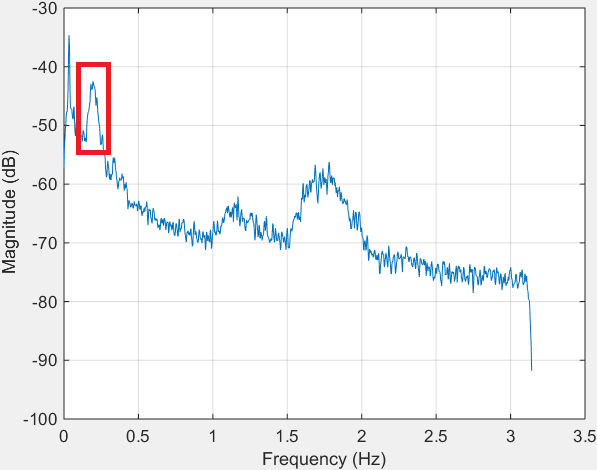
\includegraphics[width=45mm, height=35mm]{image/Ch1/1_signal.png}  \end{minipage}       &      \begin{minipage}{.3\textwidth} 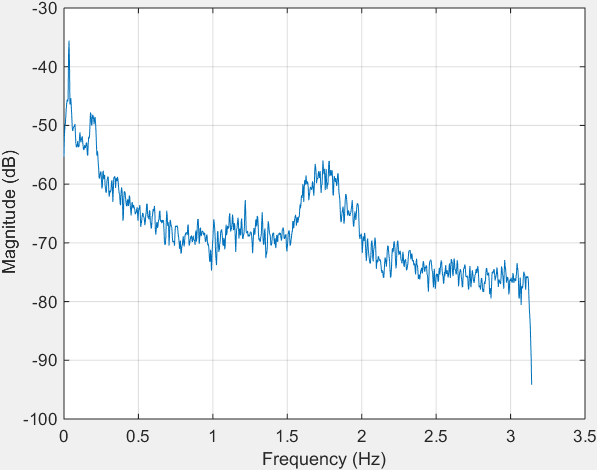
\includegraphics[width=45mm, height=35mm]{image/Ch1/1_noise.png}  \end{minipage}          \\ \hline
%\begin{tabular}[c]{@{}l@{}} \textit{Cyclorana} \\ \textit{novaehollandiae}  \end{tabular}    & \begin{minipage}{.3\textwidth} 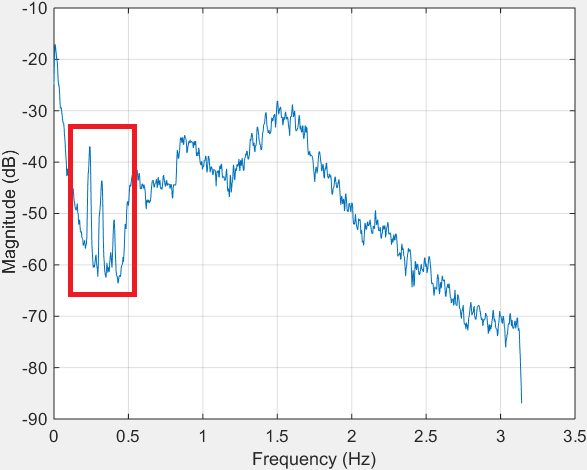
\includegraphics[width=45mm, height=35mm]{image/Ch1/2_signal.png}  \end{minipage}                              &                                              \begin{minipage}{.3\textwidth} 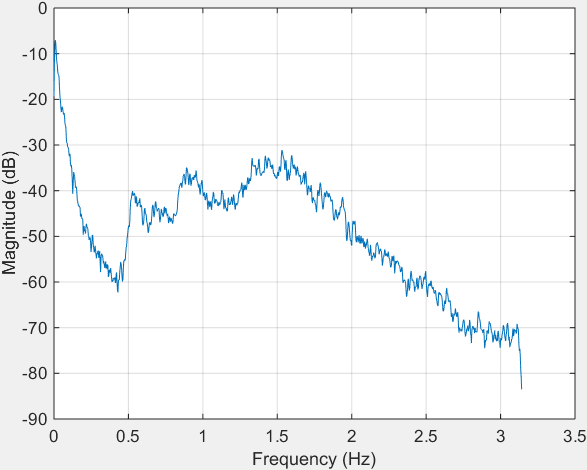
\includegraphics[width=45mm, height=35mm]{image/Ch1/2_noise.png}  \end{minipage}   \\ \hline
%
%\end{tabular}
%}
%\end{table}
%
%
%\begin{table}[htb!]
%\centering
%\resizebox{\textwidth}{!}{
%\begin{tabular}{lll}
%\hline
% \begin{tabular}[c]{@{}l@{}} \textit{Limnodynastes} \\ \textit{terraereginae}  \end{tabular}  &  \begin{minipage}{.3\textwidth} 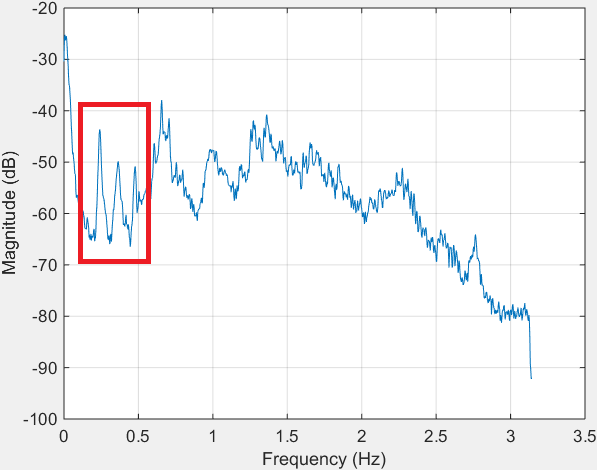
\includegraphics[width=45mm, height=35mm]{image/Ch1/3_signal.png}  \end{minipage}                              &                                             \begin{minipage}{.3\textwidth} 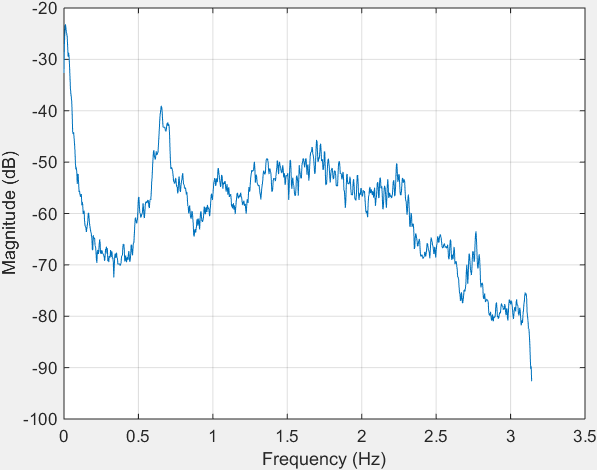
\includegraphics[width=45mm, height=35mm]{image/Ch1/3_noise.png}  \end{minipage}   \\ \hline
%\textit{Litoria fallax}              & \begin{minipage}{.3\textwidth} 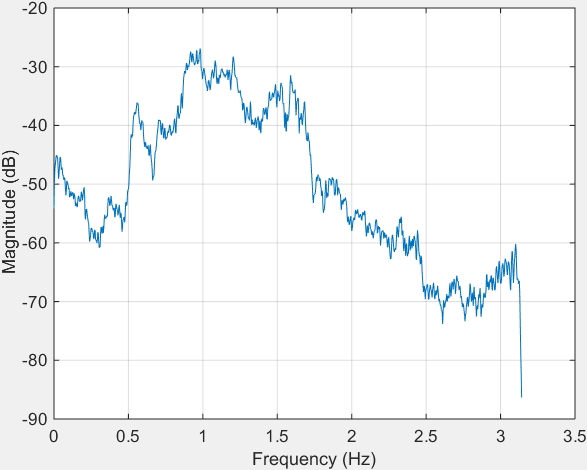
\includegraphics[width=45mm, height=35mm]{image/Ch1/4_signal.png}  \end{minipage}                             &                                               \begin{minipage}{.3\textwidth} 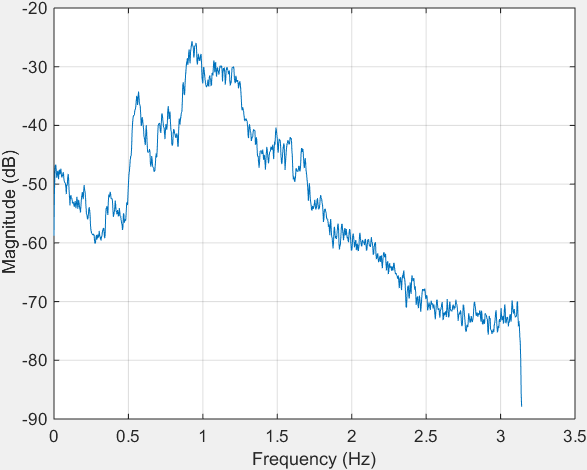
\includegraphics[width=45mm, height=35mm]{image/Ch1/4_noise.png}  \end{minipage} \\ \hline
%\textit{Litoria nasuta}              &   \begin{minipage}{.3\textwidth} 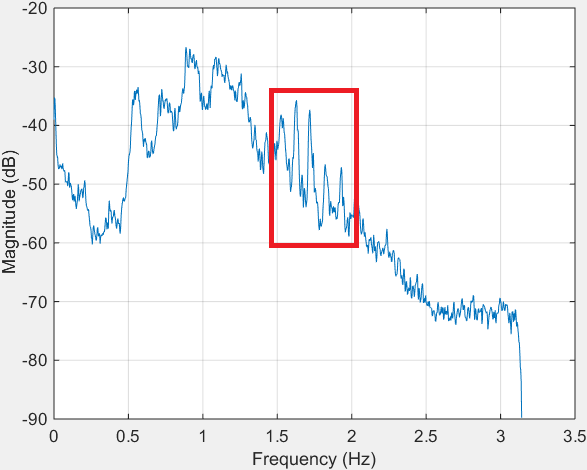
\includegraphics[width=45mm, height=35mm]{image/Ch1/5_signal.png}  \end{minipage}                           &                                               \begin{minipage}{.3\textwidth} 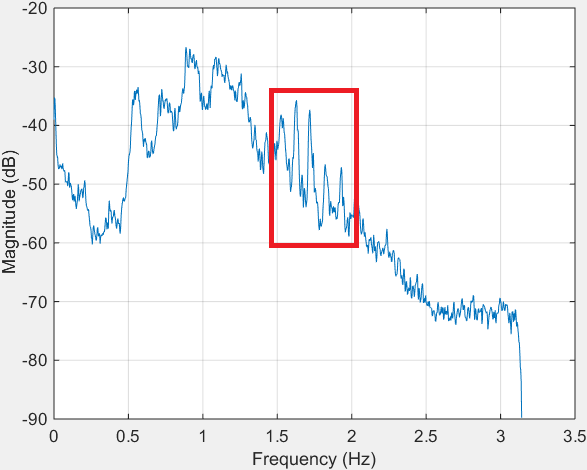
\includegraphics[width=45mm, height=35mm]{image/Ch1/5_signal.png}  \end{minipage} \\ 
%\hline
%\textit{Litoria rothii}             &  \begin{minipage}{.3\textwidth} 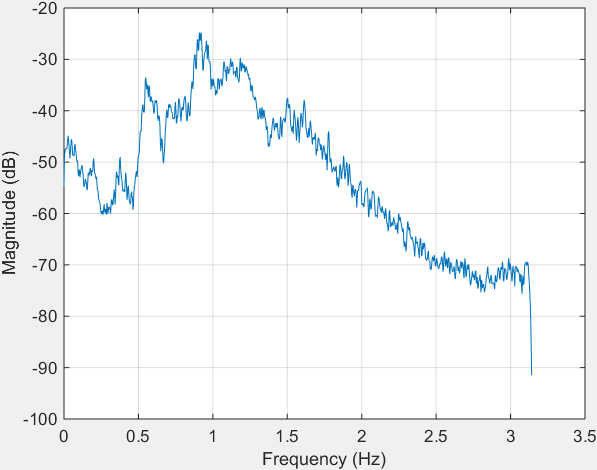
\includegraphics[width=45mm, height=35mm]{image/Ch1/6_signal.png}  \end{minipage}                         &    \begin{minipage}{.3\textwidth} 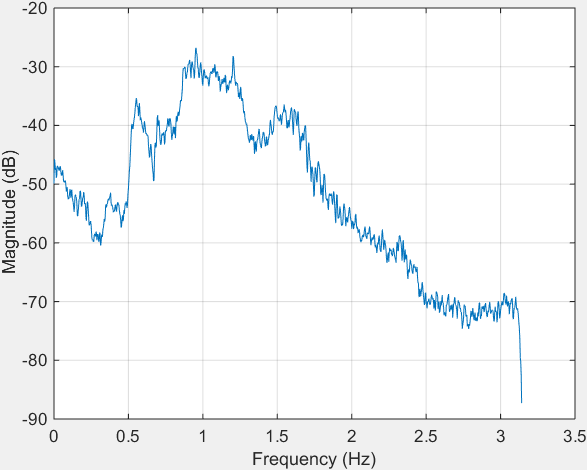
\includegraphics[width=45mm, height=35mm]{image/Ch1/6_noise.png}  \end{minipage}                                           \\ \hline
%\textit{Litoria rubella}             &    \begin{minipage}{.3\textwidth} 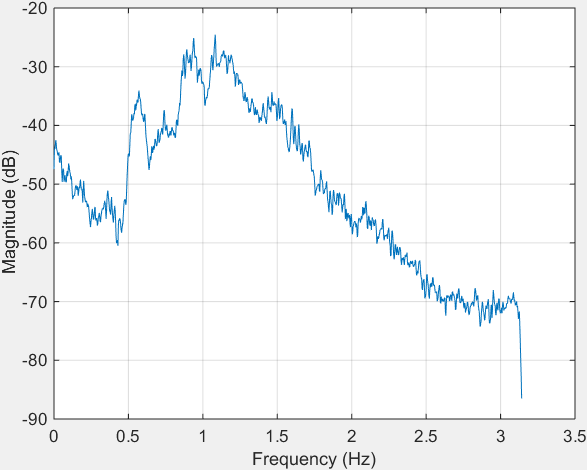
\includegraphics[width=45mm, height=35mm]{image/Ch1/7_signal.png}  \end{minipage}                               &                                               \begin{minipage}{.3\textwidth} 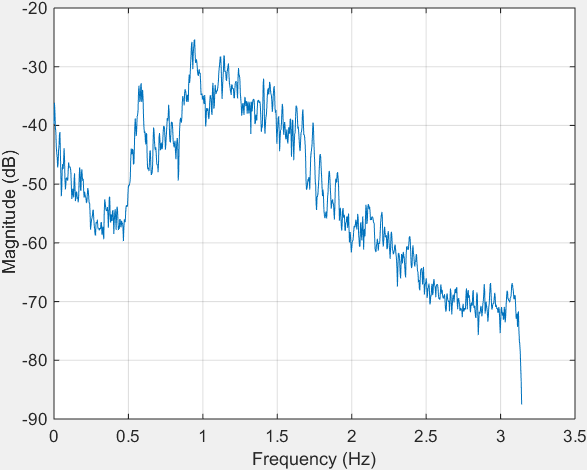
\includegraphics[width=45mm, height=35mm]{image/Ch1/7_noise.png}  \end{minipage} \\ \hline
%\textit{Uperolela mimula}            &   \begin{minipage}{.3\textwidth} 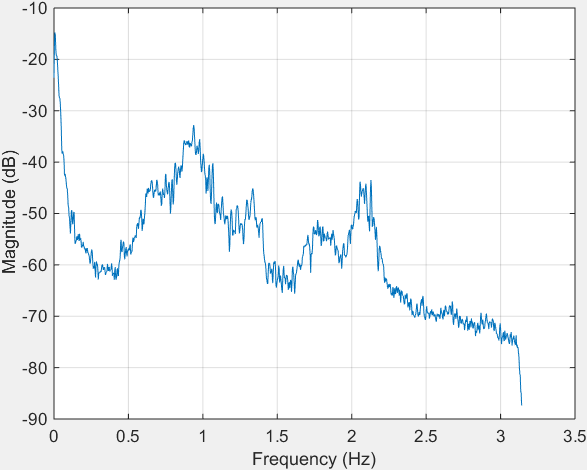
\includegraphics[width=45mm, height=35mm]{image/Ch1/8_signal.png}  \end{minipage}                              &                                             \begin{minipage}{.3\textwidth} 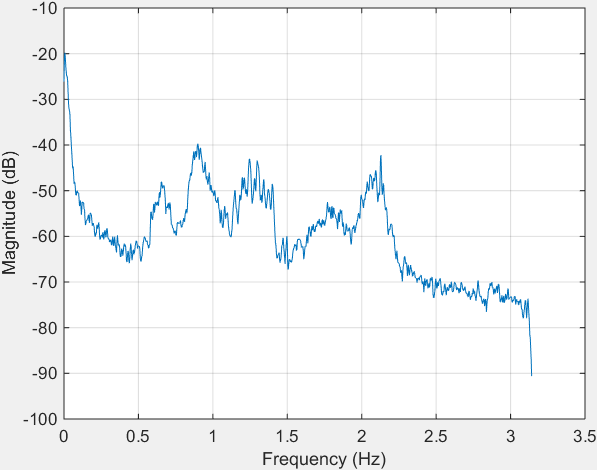
\includegraphics[width=45mm, height=35mm]{image/Ch1/8_noise.png}  \end{minipage} \\ \hline\hline
%\end{tabular}
%}
%\end{table}


%
%\appendix[Confidence interval of signal and noise]{Confidence interval of signal and noise} 
%
%
%
%
%\begin{table}[htb!]
%\centering
%\caption[Confidence interval for CD recordings]{Confidence interval of signal and noise (David Stewart's CD). The calculation of confidence interval is defined as
%$ CI=\mu \pm Z \times \frac{\sigma}{\sqrt{L}}$,where $\mu$ and $\sigma$ are the mean and standard deviation, respectively, $Z$ is the upper $\frac{(1-C)}{2}$ critical value for the standard normal distribution, $C$ is the confidence level, and set at 0.95.}
%\label{tab:CI_CD}
%\begin{tabular}{lll}
%\hline\hline
%    \backslashbox{Frog \\ species}{Parameters}                      & Confidence intervals of signal & Confidence intervals of noise \\ \hline
%\textit{Bufo marinus}        &  -9.27*$10^{-6}$ $\pm$ 2.10*$10^{-3}$ &  -2.67*$10^{-5}$ $\pm$ 2.26*$10^{-4}$                             \\ 
%\textit{Litoria caerulea}    &      -6.73*$10^{-5}$ $\pm$ 2.40*$10^{-3}$     &                              -6.89*$10^{-5}$ $\pm$ 3.90*$10^{-4}$ \\ 
%\textit{Litoria fallax}      &   -5.85*$10^{-6}$ $\pm$ 1.50*$10^{-3}$                             &                              -2.73*$10^{-5}$ $\pm$ 9.62*$10^{-6}$ \\ 
%\textit{Litoria gracillenta} &     -7.12*$10^{-5}$ $\pm$ 2.00*$10^{-3}$                           &                              -7.70* $10^{-5}$ $\pm$ 1.00*$10^{-4}$ \\ 
%\textit{Litoria latopalmata} &   -6.58*$10^{-5}$ $\pm$ 2.70*$10^{-3}$                            &                              -1.02*$10^{-4}$ $\pm$ 4.36*$10^{-5}$ \\ 
%\textit{Litoria rubella}     &   -3.13*$10^{-5}$ $\pm$ 3.00*$10^{-3}$                           &                              -9.87*$10^{-5}$ $\pm$ 4.70*$10^{-5}$ \\ \hline\hline
%\end{tabular}
%\end{table}
%
%
%
%
%\begin{table}[htb!]
%\centering
%\caption[Confidence interval for JCU recordings]{Confidence interval of signal and noise for JCU recordings}
%\label{tab:CI_JCU}
%\begin{tabular}{lll}
%\hline\hline
%   \backslashbox{Frog \\ species}{Parameters}                          & Confidence intervals of signal & Confidence intervals of noise \\ \hline
%\textit{Bufo marinus}                &   -1.36*$10^{-5}$ $\pm$ 6.00*$10^{-5}$                             &                              -3.22*$10^{-5}$ $\pm$ 4.80*$10^{-5}$ \\ \hline
%\textit{Cyclorana novaehollandiae}   &    1.30*$10^{-3}$ $\pm$ 8.70*$10^{-4}$                            &                              1.30*$10^{-3}$ $\pm$ 8.90*$10^{-4}$ \\ \hline
%\textit{Limnodynastes terraereginae} &       6.43*$10^{-5}$ $\pm$  1.30*$10^{-4}$                         &                              1.86*$10^{-4}$ $\pm$ 1.89*$10^{-4}$ \\ \hline
%\textit{Litoria fallax}              &  2.31*$10^{-5}$ $\pm$ 5.00*$10^{-4}$                              &                              5.75*$10^{-6}$ $\pm$ 4.22*$10^{-4}$ \\ \hline
%\textit{Litoria nasuta}              &                  -1.55*$10^{-4}$ $\pm$ 4.90* $10^{-4}$              &                              6.25* $10^{-6}$ $\pm$ 3.85*$10^{-4}$ \\ \hline
%\textit{Litoria rothii}              &              -3.32*$10^{-4}$ $\pm$ 9.2*$10^{-4}$                  &                              1.61* $10^{-4}$ $\pm$ 2.84*$10^{-4}$ \\ \hline
%\textit{Litoria rubella}             &      -8.15*$10^{-5}$ $\pm$ 5.52*$10^{-4}$                          &                              -2.69* $10^{-5}$ $\pm$ 4.87*$10^{-4}$ \\ \hline
%\textit{Uperolela mimula}            &             -1.20*$10^{-3}$  $\pm$ 1.10*$10^{-3}$                   &                              -9.36*$10^{-4}$ $\pm$ 3.35*$10^{-4}$ \\ \hline\hline
%\end{tabular}
%\end{table}





%\appendix[Frog species studied in this study]{Frog species studied in this study} 
%\label{app:A}







